\section{Sensors}

Sensors serve to detect both the internal condition of the robot (proprioceptive sensors) and the external state of the environment (exteroceptive sensors).
Another classification for sensors can be based on whether they are passive, which measure physical properties, or active, which involve an emitter and a detector.

\subsection{Encoder}
An encoder translates rotary motion or position of a motor/joint into electronic pulses. 
Encoders come in two primary types:
\begin{itemize}
    \item \textit{Linear encoder}: comprising a lengthy linear read track and a compact read head, linear encoders are designed for linear motion measurement.
    \item \textit{Rotary encoder}: suitable for both rotary and linear motion, rotary encoders convert rotary motion into electrical signals. 
        They are further categorized as incremental or absolute.
\end{itemize}
Their operation proceeds as follows:
\begin{enumerate}
    \item A light-emitting diode (LED) projects a light beam onto a tape striped with red and black segments.
    \item The reflected light is captured by a photodetector.
    \item The photodetector generates a periodic wave whose frequency varies based on the speed of the tape.
\end{enumerate}
\begin{figure}[H]
    \centering
    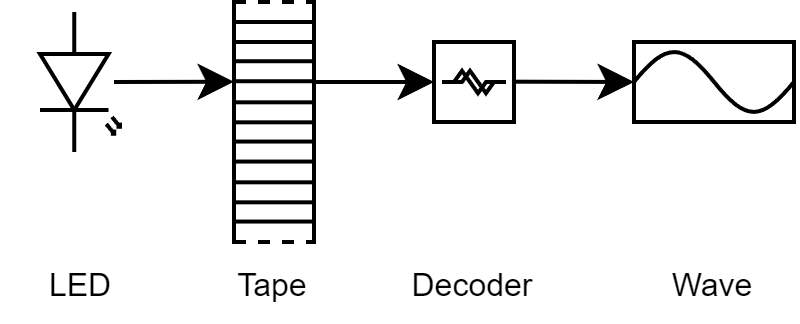
\includegraphics[width=0.6\linewidth]{images/encoder.png}
    \caption{Linear encoder structure}
\end{figure}

\paragraph*{Incremental rotary encoders}
Incremental rotary encoders operate based on the photoelectric principle, employing a disk with alternating transparent and opaque zones containing two traces or sensors.
These traces facilitate the identification of rotation direction and enhance resolution through quadrature.
\begin{figure}[H]
    \centering
    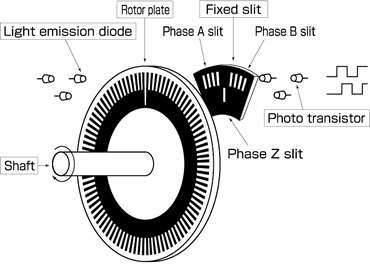
\includegraphics[width=0.35\linewidth]{images/rotary1.png}
    \caption{Incremental rotary encoder}
\end{figure}
To determine speed and direction, the quadrature technique is employed, where the two signals are shifted by $\frac{1}{4}$ step. 
Denoting $N$ as the number of steps of light/dark zones per turn, the resolution is given by:
\[\text{resolution}=\dfrac{360^{\circ}}{4N}\]
Using this technique:
\begin{itemize}
    \item If a transition from $1 1$ to $1 0$ occurs, it indicates a counterclockwise rotation.
    \item Conversely, if a transition from $1 1$ to $0 1$ occurs, it indicates a clockwise rotation.
\end{itemize}

The encoders' limitation lies in their inability to determine the actual position relative to the starting point.
The only feasible solution involves resetting to the starting position and then incrementally counting until reaching the desired position.

\paragraph*{Absolute rotary encoder}
The absolute rotary encoder addresses the limitation of determining absolute position by encoding it directly on the disk.
\begin{figure}[H]
    \centering
    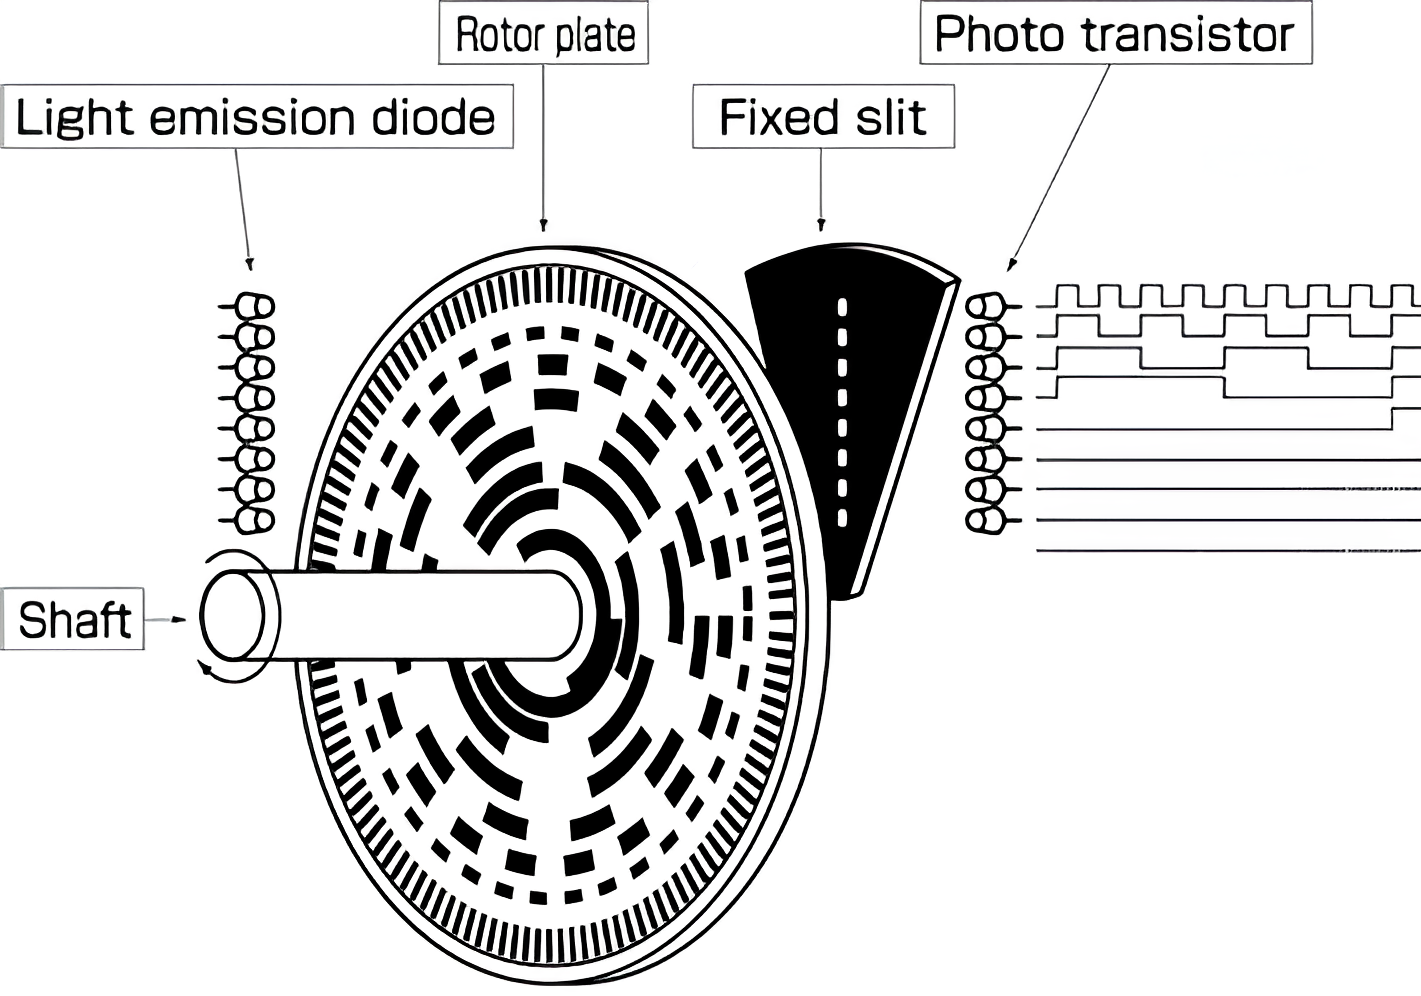
\includegraphics[width=0.35\linewidth]{images/rotary2.png}
    \caption{Incremental rotary encoder}
\end{figure}
The disk features transparent and opaque areas arranged in concentric rings. 
Each bit of position data is represented by a corresponding ring, offering an absolute resolution of:
\[\text{resolution}=\dfrac{360^{\circ}}{2^N}\]
In robotic applications, a minimum of 12 rings are typically employed. 
To prevent ambiguities, binary codes with single variations, such as Gray code, are utilized.

\subsection{Time of flight telemeter}
The time-of-flight telemeter records the duration between when the emitter generates a signal and when the detector detects its reflection.
The signal travels a distance of $2d$, and the time of flight is given by: 
\[\Delta t=\dfrac{2d}{c}\]
The initial type of sensor utilizing this principle in robotics was the sonar, which relies on sound waves.
Sound waves, with their slower speed of approximately $340\:m/s$, and their relatively broad directionality ranging from $20^{\circ}$ to $40^{\circ}$, offer an advantage in measuring shorter distances.
\begin{figure}[H]
    \centering
    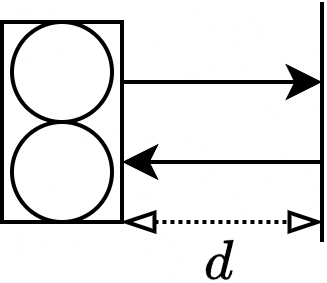
\includegraphics[width=0.2\linewidth]{images/sonar.png}
    \caption{Sonar sensor}
\end{figure}
\begin{table}[H]
    \centering
    \begin{tabular}{ll}
    \multicolumn{2}{c}{\textbf{Sonar}}                                   \\ \hline
    \multicolumn{1}{l|}{\textit{Range (m)}}               & 0.3 up to 10 \\
    \multicolumn{1}{l|}{\textit{Accuracy (m)}}            & 0.025        \\
    \multicolumn{1}{l|}{\textit{Cone opening ($\:^\circ$)}} & 30           \\
    \multicolumn{1}{l|}{\textit{Frequency (Hz)}}          & 50000       
    \end{tabular}
\end{table}
The primary limitation is the susceptibility of the signal-to-noise, particularly from significant reflections.
Selecting an appropriate range is crucial depending on the specific application. 
However, these sensors may not function optimally in all scenarios, due to factors such as:
\begin{itemize}
    \item Balancing sampling frequency. 
    \item Dealing with reflections off walls. 
    \item Detecting small or soft objects. 
\end{itemize}
Additionally, it's worth noting that room dimensions may appear distorted, especially around corners.
\begin{figure}[H]
    \centering
    \begin{subfigure}{0.3\textwidth}
        \centering
        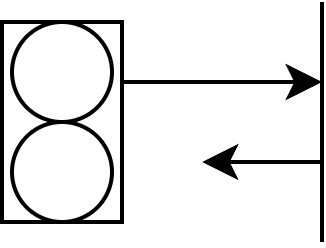
\includegraphics[width=0.5\linewidth]{images/far.png} 
        \caption{Distance}
    \end{subfigure}
    \begin{subfigure}{0.3\textwidth}
        \centering
        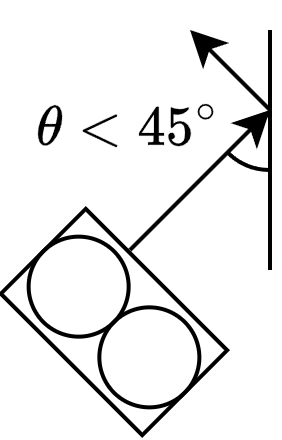
\includegraphics[width=0.4\linewidth]{images/inclination.png}
        \caption{Inclination}
    \end{subfigure}
    \begin{subfigure}{0.3\textwidth}
        \centering
        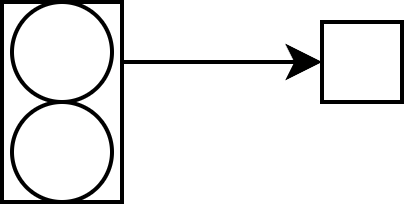
\includegraphics[width=0.6\linewidth]{images/dimension.png} 
        \caption{Dimension}
    \end{subfigure}
    \caption{Possible problems for sonar sensors}
\end{figure}

\subsection{Reflective optosensors}
Reflective optosensors are active sensors where the emitter is a source of light and the detector is a light detector. 
This type of sensors uses triangulation to compute distance: 
\begin{enumerate}
    \item Emitter casts a beam of light on the surface. 
    \item The detector measures the angle corresponding to the maximum intensity of returned light. 
    \item Being $s$ the distance between the emitter and the detector we have: 
    \[d=s \cdot \tan \alpha\]
\end{enumerate}
\begin{figure}[H]
    \centering
    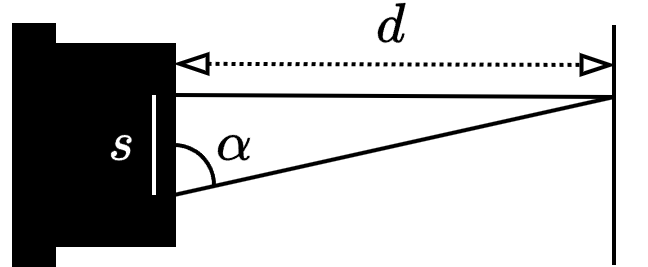
\includegraphics[width=0.35\linewidth]{images/opto.png}
    \caption{Reflective optosensor}
\end{figure}
Infrared sensors are relatively inexpensive and sturdy, but they have their drawbacks. 
They exhibit nonlinear characteristics that require calibration.
Additionally, there can be ambiguity when used at short ranges, necessitating precise placement within the robot. 
Their fixed ranges and opening angles mean that careful selection is needed for optimal performance in various applications. 
Moreover, they may encounter issues with reflections under certain conditions.

An instance of such technology is the Kinect, an input device designed by Microsoft (originally by Primesense) for Xbox 360.
This device functions as a three-dimensional scanner and is equipped with an infrared projector, an infrared camera, and an RGB camera.
\begin{table}[H]
    \centering
    \begin{tabular}{ll}
    \multicolumn{2}{c}{\textbf{Kinect}}                                                         \\ \hline
    \multicolumn{1}{l|}{\textit{Range (m)}}                             & 0.7 up to 6           \\
    \multicolumn{1}{l|}{\textit{Horizontal cone opening ($\:^\circ$)}}  & 57                    \\
    \multicolumn{1}{l|}{\textit{Vertical cone opening ($\:^\circ$)}}    & 43                    \\
    \multicolumn{1}{l|}{\textit{Infrared camera}}                       & 11-bit 640$\times$480        \\    
    \multicolumn{1}{l|}{\textit{RGB camera}}                            & $30\:Hz$ 8-bit 640$\times$480    \\  
    \end{tabular}
\end{table}
In this device, the distance from the camera $Z_k$ is calculated as:
\[Z_k=\dfrac{Z_0}{1+\dfrac{d}{fb}Z_0}\]

\paragraph*{Time of flight camera}
Three-dimensional time-of-flight (TOF) cameras illuminate the scene using a modulated light source and capture the reflected light. 
The phase shift between illumination and reflection is then translated into distance information.

These sensors encounter challenges such as utilizing illumination from a solid-state laser or a near-infrared ($\sim 850 \: nm$) LED, where an imaging sensor converts captured light into electrical current. 
Additionally, distance information is encoded within the reflected component. 
Consequently, a high ambient component diminishes the signal-to-noise ratio (SNR).

\subsection{Light detection and ranging (LIDAR)}
Laser sensors offer superior accuracy with the following capabilities:
\begin{itemize}
    \item Providing 180 ranges across a 180° field of view (expandable to 360°).
    \item Scanning 1 to 64 planes.
    \item Delivering scan rates of 10-75 scans per second.
    \item Achieving range resolutions of less than $1\:cm$.
    \item Offering a maximum range of up to 50-80 meters.
    \item Facing challenges only with mirrors, glass, and matte black surfaces.
\end{itemize}

\subsection{Position sensor}
Positioning outdoors can be determined using a Global Navigation Satellite System (GNSS), with multiple constellations available including GPS, GLONASS, Beidou, Galileo, and more.

The Global Positioning System (GPS) comprises 24 satellites circling the Earth twice daily. 
These satellites emit synchronized signals containing location and time data.
Receivers compare the transmitted and received signal times to determine position.
At least four satellite signals are needed for accurate positioning.
The typical accuracy of GPS is approximately $2.5\:m$ at a $2\:Hz$ refresh rate, with the potential for even greater precision of around $20\:cm$ with Differential GPS (DGPS).

There is also the RTKGPS that improves the time resolution with respect to the DGPS.

There are several limitations associated with GPS:
\begin{itemize}
    \item It does not function indoors, underwater, or in urban canyons.
    \item Line of sight reception is required for optimal performance.
    \item GPS signals are susceptible to multiple paths and reflections, which can affect accuracy.
\end{itemize}

\section{Inertial sensor}
The inertial sensor can be divided into the following categories:
\begin{itemize}
    \item \textit{Gyroscopes}: measure angular velocities.
    \item \textit{Accelerometers}: gauge linear accelerations with reference to the gravitational vector.
    \item \textit{Magnetometers/compasses}: determine orientation based on the earth's magnetic field vector.
\end{itemize}
An Inertial Measurement Unit (IMU) integrates gyroscopes, accelerometers, and magnetometers to offer a complete six degrees of freedom pose estimate. 
However, integrating inertial measurements, such as for position computation, accumulates errors and drifts notably over time, particularly when using inexpensive MEMS (Micro-Electro-Mechanical Systems) technology.

\subsection{Tactile sensor}
Tactile sensors serve manipulation purposes and fall into two main categories:
\begin{itemize}
    \item \textit{Binary}: utilize switches placed on the fingers of a manipulator.
        Can be arranged in arrays (bumpers) on the external side to detect and avoid obstacles.
    \item \textit{Analogical} (real valued): consist of soft devices producing a signal proportional to the local force.
        Utilize mechanisms like a spring coupled with a shaft or soft conductive material that changes resistance with compression.
        Capable of measuring movements tangential to the sensor surface.
\end{itemize}

\subsection{Proximity sensor}
Proximity sensors detect the presence of objects within a defined distance range, employed for grasping items and navigating around obstacles. 
Various technologies are utilized for this purpose:
\begin{itemize}
    \item \textit{Ultrasonic}: low cost.
    \item \textit{Inductive}: detects ferromagnetic materials within a millimeters distance.
    \item \textit{Hall effect}: detects ferromagnetic materials, small, robust, and inexpensive.
    \item \textit{Capacitive}: detects any object, binary output, high accuracy when calibrated for a specific object.
    \item \textit{Optical}: utilizes infrared light, offering binary or real-valued output.
\end{itemize}